%% ------------------------------------------------------------------------- %%
\chapter{Methods, Results, and Conclusion}
\label{cap:conclusoes}

\section{Methods}

Matrix norms were used to assert the correctness of our results. 
Let %$x \in \Cfield^n$ and 
$A \in \Cfield^{m \times n}$. \cite{watkins:2004} defines  
matrix 1-norm as:
\begin{equation}
%	\norm{x}_{\infty} = \max\limits_{1 \leq k \leq n} |x_k| \qquad 
%	\norm{A}_{\infty} = \max\limits_{1 \leq i \leq m} \sum_{j=1}^{n} |a_{ij}| \quad
	\norm{A}_{   1  } = \max\limits_{1 \leq j \leq n} \sum_{i=1}^{m} |a_{ij}| \quad
\end{equation}

All norms have the property that $\norm{A} = 0$ if and only if $A = 0$.
Let $u$ and $v$ be two numerical 
algorithms that solve the same problem, but in a different way. 
Now let $y_u$ be the result computed by $u$ and $y_v$ be the result computed by
$v$. The \textit{error} between these two values can be measured computing
$\norm{y_u - y_v}$. The error between CPU and GPU versions of $H$ and $G$ matrices was computed by calculating $\norm{H_{cpu} - H_{gpu}}_1$
and $\norm{G_{cpu} - G_{gpu}}_1$. An automated test check if this value is bellow $10^{-4}$.

Gfortran 5.4.0 and CUDA 8.0 were used to compile the application. The main flags used in Gfortran were
$\texttt{-Ofast}$ $\texttt{-march=native}$ $\texttt{-funroll-loops}$ $\texttt{-flto}$. The flags used in
CUDA nvcc compiler were: $\texttt{-use\_fast\_math}$  $\texttt{-O3}$ $\texttt{-Xptxas}$ $\texttt{--opt-level=3}$
$\texttt{-maxrregcount=32}$ $\texttt{-Xptxas}$ 
$\texttt{--allow-expensive-optimizations=true}$ . 

For experimenting, there were four data samples as shown in Table \ref{experiments}. The application was 
executed for each sample using the original code (serial implementation), the OpenMP 
version and the CUDA and OpenMP together. All tests but the sequential set the number of OpenMP 
threads to 4. The machine used in all experiments had an AMD A10-7700K processor paired with a 
GeForce GTX980\footnote{Thanks to NVIDIA for donating this GPU.}.

Before any data collection, a warm up procedure is executed, which consists of running the 
application with the sample three times without getting any result. Afterward, all experiments 
were executed 30 times per sample. Each execution produced a file with total time elapsed, 
where a script computed averages and standard deviations for all experiments.

GPU total time was computed by the sum of 5 elements: 
(1) total time to move data to GPU, (2) launch and execute the kernel, (3) elapsed time 
to compute the result, (4) time to move data back to main memory, (5) time to compute 
the remaining $H$ and $G$ parts in the CPU. 
The elapsed time was computed in seconds with the OpenMP library function 
$\texttt{OMP\_GET\_WTIME}$. This function calculates the elapsed wall clock time in seconds 
with double precision. All experiments set the Gauss Quadrature Points to 8.

\begin{table}[]
\centering
\caption{Data experiment set}
\label{experiments}
\begin{tabular}{|l|l|l|l|l|}
\hline
Number of Mesh elements     & 240 & 960 & 2160 & 4000 \\ \hline
Number of Boundary elements & 100 & 400 & 900  & 1600 \\ \hline
\end{tabular}
\end{table}

\section{Results}


The logarithmic scale graphic at Figure 1 illustrates the results. All points are the mean of the 
time in seconds of 30 executions as described in Methodology. The average is meaningful as the maximum standard deviation
obtained was $2.6\%$ of the mean value.

\begin{figure}[ht]
\centering
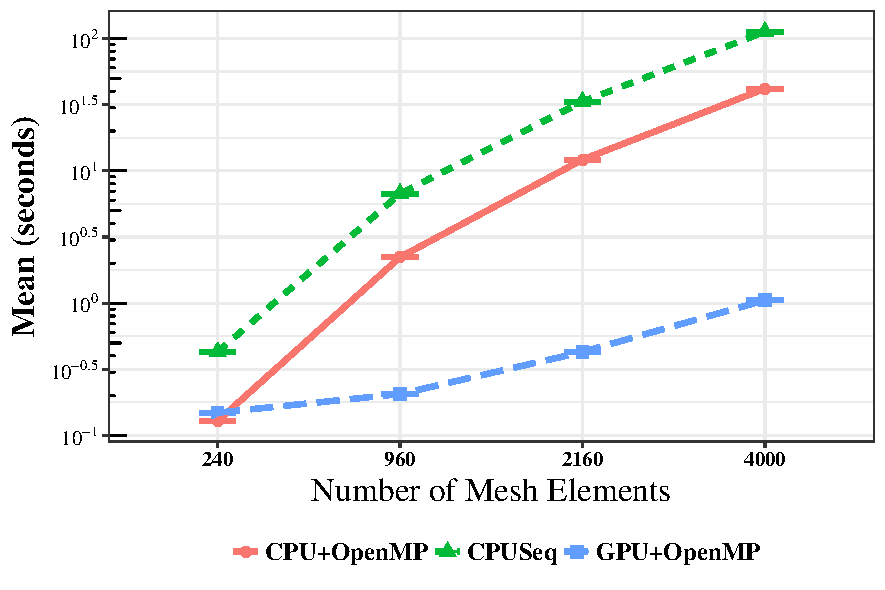
\includegraphics[scale=0.866]{results1.pdf}
\caption{Time elapsed by each implementation in logarithm scale}
\label{fig:graphic1}
\end{figure}

The speedup acquired in the $4000$ mesh elements sample with OpenMP and CUDA+OpenMP with respect to the sequential 
algorithm are $2.7$ and $107$ respectively. As a conclusion, the presented strategy paired with GPUs can be 
used to accelerate the overall performance of the simulation for a large number of mesh elements. This is a consequence 
of parallelizing the construction of both matrices $H$ and $G$, and the calculations in the $\texttt{Nonsingd}$ routine. 
Notice that there was a performance loss in the 260 sample between OpenMP and CUDA+OpenMP, this was caused by the high 
latency between CPU-GPU communication, thus the usage of GPUs may not be attractive for small meshes.
